\documentclass[a4paper]{article}
\usepackage[a4paper,margin=0mm]{geometry}
\usepackage{fontspec}
\usepackage{unicode-math}
\usepackage{tikz}
\usetikzlibrary{fit,calc,positioning,arrows.meta}
\usepackage[table]{xcolor}
\usepackage[absolute]{textpos}
\usepackage{array}

\setmainfont{Libertinus Serif}
\setsansfont{Libertinus Sans}
\setmathfont{Libertinus Math}

\definecolor{accent}{HTML}{602785}
\definecolor{badge}{HTML}{B8A0C8}
\definecolor{ink}{HTML}{2A2E30}
\definecolor{warn}{HTML}{3D1856}

\setlength{\TPHorizModule}{1mm}
\setlength{\TPVertModule}{1mm}
\setlength{\parindent}{0pt}
\pagestyle{empty}

\newcommand{\topicheader}[2]{%
\begin{textblock*}{194mm}(16mm,10mm)
\begin{tikzpicture}
\node[fill=accent,text=white,font=\sffamily\bfseries\fontsize{13}{13}\selectfont,
      minimum width=9mm,minimum height=9mm,inner sep=0pt] at (4.5mm,-4.5mm) {#1};
\node[font=\sffamily\bfseries\fontsize{15}{16}\selectfont,text=ink,anchor=west] at (12mm,-4.5mm) {#2};
\end{tikzpicture}
\end{textblock*}
\begin{textblock*}{194mm}(16mm,22.5mm)

\begin{tikzpicture}
\fill[accent] (0,0) rectangle (194mm,0.5mm);
\end{tikzpicture}
\end{textblock*}
}

\newcommand{\pagekicker}[1]{%
\begin{textblock*}{100mm}(16mm,25.5mm)
\begin{tikzpicture}
\node[fill=ink,text=white,font=\sffamily\bfseries\fontsize{8}{8}\selectfont,
      inner sep=2.2pt,rounded corners=1pt] {\MakeUppercase{#1}};
\end{tikzpicture}
\end{textblock*}
}

\newcommand{\videobanner}[1]{%
\begin{textblock*}{178mm}(16mm,25.5mm)
\begin{tikzpicture}
\fill[accent] (0,0) rectangle (178mm,-10mm);
\draw[white,line width=0.6pt] (3mm,-1.7mm) rectangle (11.5mm,-8.3mm);
\node[white,font=\sffamily\fontsize{4}{4.4}\selectfont,align=center] at (7.25mm,-5mm) {QR\\CODE};
\node[white,font=\sffamily\bfseries\fontsize{9.5}{11}\selectfont,anchor=west] at (16mm,-5.6mm) {WATCH THE VIDEO BEFORE YOU SOLVE};
\node[white,font=\sffamily\fontsize{7.5}{8}\selectfont,anchor=east] at (174mm,-5.6mm) {YouTube ~\textbullet~ #1};
\end{tikzpicture}
\end{textblock*}
}

\newcommand{\pagefooter}[1]{%
\begin{textblock*}{194mm}(8mm,286.41mm)
  
\begin{tikzpicture}
    \fill[accent] (0,0) rectangle (194mm,0.6mm);
  \end{tikzpicture}
\end{textblock*}
\begin{textblock*}{63.59mm}(8mm,288.27mm)
  {\sffamily\bfseries\color{accent}\fontsize{13}{16}\selectfont SAT 1200+}
\end{textblock*}
\begin{textblock*}{10mm}(188mm,288.27mm)
  \centering{\sffamily\color{accent}\fontsize{14}{16}\selectfont #1}
\end{textblock*}
}

\newcommand{\cardbg}[4]{%
\begin{textblock*}{#3mm}(#1mm,#2mm)
\begin{tikzpicture}
\fill[badge!22,rounded corners=3mm] (0,0) rectangle (#3mm,-#4mm);
\end{tikzpicture}
\end{textblock*}%
}

\newcommand{\warnbgbox}[4]{%
\begin{textblock*}{#3mm}(#1mm,#2mm)
\begin{tikzpicture}
\fill[badge!38,rounded corners=3mm] (0,0) rectangle (#3mm,-#4mm);
\draw[warn,line width=1pt,rounded corners=3mm] (0,0) rectangle (#3mm,-#4mm);
\end{tikzpicture}
\end{textblock*}%
}

\newcommand{\pill}[3]{%
\begin{textblock*}{160mm}(#1mm,#2mm)
\begin{tikzpicture}
\node[fill=accent,text=white,anchor=north west,font=\sffamily\bfseries\fontsize{10}{10}\selectfont,
      rounded corners=8pt,inner xsep=5mm,inner ysep=1.8mm] at (0,0) {RULE ~\textperiodcentered~ #3};
\end{tikzpicture}
\end{textblock*}%
}

\newcommand{\pillwarn}[3]{%
\begin{textblock*}{160mm}(#1mm,#2mm)
\begin{tikzpicture}
\node[fill=warn,text=white,anchor=north west,font=\sffamily\bfseries\fontsize{10}{10}\selectfont,
      rounded corners=8pt,inner xsep=5mm,inner ysep=1.8mm] at (0,0) {WARNING ~\textperiodcentered~ #3};
\end{tikzpicture}
\end{textblock*}%
}

\arrayrulecolor{accent}
\setlength{\arrayrulewidth}{0.7pt}
\renewcommand{\arraystretch}{1.5}

\begin{document}

% ======================================================================
% PAGE 1
% ======================================================================
\topicheader{3}{Linear Functions \& Graphing}
\videobanner{Lesson 3}
\pagefooter{17}
\mbox{}%

% ---- CARD 1: Slope ----
\cardbg{16}{40}{178}{90}
\pill{26}{43}{Slope (qiyalik)}

\begin{textblock*}{158mm}(26mm,56mm)
{\fontsize{13}{15}\selectfont $m=\dfrac{y_2-y_1}{x_2-x_1}$}
\end{textblock*}

\begin{textblock*}{100mm}(26mm,73mm)
{\fontsize{10}{13}\selectfont\color{ink}
\textbf{Term bridge:} traditional textbooks call this $k$ (and $y=kx+b$);
the SAT calls it \textbf{slope} and $m$ (and $y=mx+b$) -- same thing.\\[2mm]
\textbf{Example:} through $(3,2)$ and $(7,10)$:\\
$m=\dfrac{10-2}{7-3}=\dfrac{8}{4}=2$}
\end{textblock*}

\begin{textblock*}{60mm}(128mm,73mm)
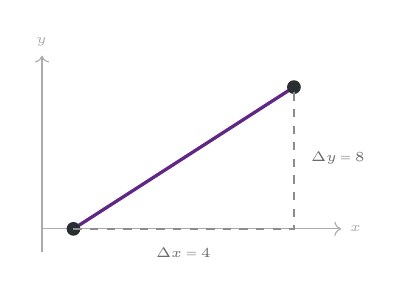
\begin{tikzpicture}
\draw[ink!40,->] (0,0) -- (38mm,0) node[right,font=\tiny]{$x$};
\draw[ink!40,->] (0,-3mm) -- (0,22mm) node[above,font=\tiny]{$y$};
\draw[accent,line width=1.2pt] (4mm,0) -- (32mm,18mm);
\filldraw[ink] (4mm,0) circle (0.8mm);
\filldraw[ink] (32mm,18mm) circle (0.8mm);
\draw[ink!55,dashed,line width=0.6pt] (4mm,0) -- (32mm,0) -- (32mm,18mm);
\node[font=\sffamily\tiny,text=ink!70] at (18mm,-3mm) {$\Delta x=4$};
\node[font=\sffamily\tiny,text=ink!70,anchor=west] at (33mm,9mm) {$\Delta y=8$};
\end{tikzpicture}
\end{textblock*}

\begin{textblock*}{158mm}(26mm,110mm)
{\fontsize{10.5}{13}\selectfont\color{ink}
\textbf{In $y=mx+b$:} $m$ is the slope, $b$ is the $y$-intercept. Don't mix
them up: in $y=5x-3$, slope is $5$, $y$-intercept is $-3$.}
\end{textblock*}

% ---- CARD 2: WARNING -- inverted formula ----
\warnbgbox{16}{134}{178}{44}
\pillwarn{26}{137}{Don't invert the formula}

\begin{textblock*}{158mm}(26mm,149mm)
{\fontsize{10.5}{13}\selectfont\color{ink}
Always \textbf{rise ($y$) over run ($x$)}: $m=\dfrac{y_2-y_1}{x_2-x_1}$ --
\textbf{never} $\dfrac{x_2-x_1}{y_2-y_1}$.}
\end{textblock*}

% ---- CARD 3: Point-slope form ----
\cardbg{16}{184}{178}{100}
\pill{26}{187}{Writing a line's equation}

\begin{textblock*}{158mm}(26mm,200mm)
{\fontsize{12}{14}\selectfont Point-slope form: $y-y_1=m(x-x_1)$}
\end{textblock*}

\begin{textblock*}{158mm}(26mm,211mm)
{\fontsize{10}{13}\selectfont\color{ink}
\textbf{Slope $4$, point $(1,3)$:}\\
$y-3=4(x-1)\ \Rightarrow\ y-3=4x-4\ \Rightarrow\ y=4x-1$}
\end{textblock*}

\begin{textblock*}{158mm}(26mm,229mm)
{\fontsize{10}{13}\selectfont\color{ink}
\textbf{Two points $(2,1)$ and $(4,7)$:} find $m$ first:
$m=\dfrac{7-1}{4-2}=3$; then use $(2,1)$:\\
$y-1=3(x-2)\ \Rightarrow\ y-1=3x-6\ \Rightarrow\ y=3x-5$}
\end{textblock*}

\begin{textblock*}{158mm}(26mm,268mm)
{\fontsize{9.5}{12}\selectfont\color{black!55}\itshape
Slope-intercept form ($y=mx+b$) is best for graphing and reading the slope;
point-slope form is best for starting from a point and a slope.}
\end{textblock*}

\clearpage

% ======================================================================
% PAGE 2
% ======================================================================
\topicheader{3}{Linear Functions \& Graphing}
\pagekicker{Rules sheet -- 2/2}
\pagefooter{18}
\mbox{}%

% ---- CARD 4: Parallel and perpendicular ----
\cardbg{16}{33}{178}{98}
\pill{26}{36}{Parallel \& perpendicular lines}

\begin{textblock*}{158mm}(26mm,49mm)
{\fontsize{12}{14}\selectfont
$m_1=m_2$ (parallel) \hspace{10mm} $m_1\times m_2=-1$ (perpendicular)}
\end{textblock*}

\begin{textblock*}{95mm}(26mm,62mm)
{\fontsize{10}{13}\selectfont\color{ink}
\textbf{Perpendicular to $y=2x-5$, through $(4,1)$:}\\
Negative reciprocal of slope $2$: $-\dfrac12$.\\
$y-1=-\dfrac12(x-4)\ \Rightarrow\ y=-\dfrac12x+3$}
\end{textblock*}

\begin{textblock*}{55mm}(125mm,63mm)
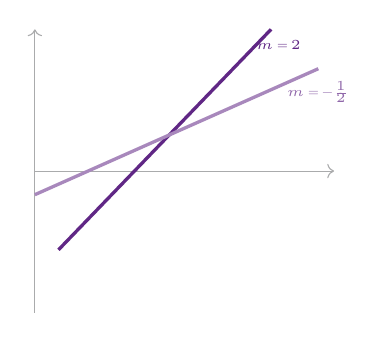
\begin{tikzpicture}
\draw[ink!40,->] (0,0) -- (38mm,0); \draw[ink!40,->] (0,-18mm) -- (0,18mm);
\draw[accent,line width=1.2pt] (3mm,-10mm) -- (30mm,18mm);
\draw[accent!55,line width=1.2pt] (0,-3mm) -- (36mm,13mm);
\node[font=\sffamily\tiny,text=accent] at (31mm,16mm) {$m=2$};
\node[font=\sffamily\tiny,text=accent!70] at (36mm,10mm) {$m=-\frac12$};
\end{tikzpicture}
\end{textblock*}

\begin{textblock*}{158mm}(26mm,98mm)
{\fontsize{10.5}{13}\selectfont\color{ink}
\textbf{Parallel lines} -- same slope, different $y$-intercept (never
cross). \textbf{Perpendicular} -- cross at a right angle.}
\end{textblock*}

\begin{textblock*}{50mm}(26mm,112mm)
{\centering\fontsize{9}{9}\selectfont\textbf{Parallel}\par}
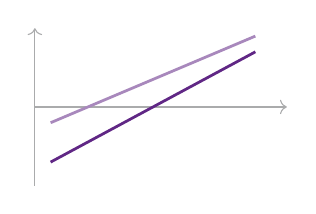
\begin{tikzpicture}
\draw[ink!40,->] (0,0) -- (32mm,0); \draw[ink!40,->] (0,-10mm) -- (0,10mm);
\draw[accent,line width=1pt] (2mm,-7mm) -- (28mm,7mm);
\draw[accent!55,line width=1pt] (2mm,-2mm) -- (28mm,9mm);
\end{tikzpicture}
\end{textblock*}

\begin{textblock*}{50mm}(110mm,112mm)
{\centering\fontsize{9}{9}\selectfont\textbf{Perpendicular}\par}
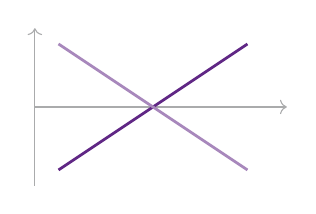
\begin{tikzpicture}
\draw[ink!40,->] (0,0) -- (32mm,0); \draw[ink!40,->] (0,-10mm) -- (0,10mm);
\draw[accent,line width=1pt] (3mm,-8mm) -- (27mm,8mm);
\draw[accent!55,line width=1pt] (3mm,8mm) -- (27mm,-8mm);
\end{tikzpicture}
\end{textblock*}

% ---- CARD 5: WARNING -- negative reciprocal ----
\warnbgbox{16}{137}{178}{42}
\pillwarn{26}{140}{Flip AND negate}

\begin{textblock*}{158mm}(26mm,152mm)
{\fontsize{10.5}{13}\selectfont\color{ink}
A perpendicular slope is both flipped and sign-reversed:
$\dfrac23 \to -\dfrac32$ -- don't just flip and forget the sign.}
\end{textblock*}

% ---- CARD 6: Real-world meaning ----
\cardbg{16}{185}{178}{95}
\pill{26}{188}{Real-world meaning of slope \& intercept}

\begin{textblock*}{158mm}(26mm,201mm)
{\fontsize{10.5}{13}\selectfont\color{ink}
In a word problem: \textbf{slope} = rate of change (per unit), \textbf{$y$-intercept}
= starting value (at $x=0$).\\[2mm]
\textbf{Example:} $C(x)=2000x+5000$ (taxi fare, $x$ = km). $C(10)=2000(10)+5000=25000$
som. ($2000$ = price per km; $5000$ = starting fee.)}
\end{textblock*}

\begin{textblock*}{158mm}(26mm,236mm)
{\fontsize{10}{13}\selectfont\color{warn}\sffamily\bfseries WARNING:}
{\fontsize{10}{13}\selectfont\color{ink}
read the question fully -- is it asking for the slope itself, the value at
a given $x$, or $x$ itself? Each needs a different move.}
\end{textblock*}

\begin{textblock*}{158mm}(26mm,262mm)
{\fontsize{9.5}{12}\selectfont\color{black!55}\itshape
The sign matters too: a negative slope means decrease (e.g. water draining
from a tank), a positive slope means increase.}
\end{textblock*}

\end{document}
